\documentclass[11pt]{article}
\usepackage[margin=1in]{geometry}
\usepackage{booktabs}
\usepackage{longtable}
\usepackage{array}
\usepackage{amsmath}
\usepackage{graphicx}
\usepackage{hyperref}
\hypersetup{colorlinks=true, linkcolor=blue, urlcolor=blue}
\sloppy
\newcolumntype{L}[1]{>{\raggedright\arraybackslash}p{#1}}

% Every number in this document is defined by analyze_permit_content.py in the two
% generated files below. Nothing is typed by hand.
% GENERATED BY analyze_permit_content.py --- do not edit by hand.
\newcommand{\pcCellDaysMedB}{303}
\newcommand{\pcCellMedGap}{197}
\newcommand{\pcCols}{57}
\newcommand{\pcCompleteNoDate}{0.00}
\newcommand{\pcCostNominal}{1}
\newcommand{\pcCostPlaceholder}{10.2}
\newcommand{\pcCostPlaceholderLinked}{1.8}
\newcommand{\pcCostPlaceholderUnlinked}{2.0}
\newcommand{\pcCostQ}{5}
\newcommand{\pcCostQAltHi}{10}
\newcommand{\pcCostQAltLo}{2}
\newcommand{\pcDataCols}{53}
\newcommand{\pcDrBothN}{2{,}269}
\newcommand{\pcDrCases}{2{,}524}
\newcommand{\pcDrDbiMed}{294}
\newcommand{\pcDrDbiN}{2{,}356}
\newcommand{\pcDrDbiNeg}{3.0}
\newcommand{\pcDrDbiPninety}{791}
\newcommand{\pcDrDiffMed}{150}
\newcommand{\pcDrFiled}{2006--2020}
\newcommand{\pcDrNamedInDbi}{487}
\newcommand{\pcDrNegN}{201}
\newcommand{\pcDrNegOffParcel}{18}
\newcommand{\pcDrNegOwn}{110}
\newcommand{\pcDrNegPct}{8.9}
\newcommand{\pcDrNegRecord}{76}
\newcommand{\pcDrNegStem}{15}
\newcommand{\pcDrNegStemOff}{2}
\newcommand{\pcDrRecMed}{101}
\newcommand{\pcDrRecN}{2{,}418}
\newcommand{\pcDrRecPninety}{315}
\newcommand{\pcDrpN}{693}
\newcommand{\pcDrpNamed}{646}
\newcommand{\pcDrpYears}{2015--2020}
\newcommand{\pcDupIds}{0}
\newcommand{\pcFcdFilled}{1.2}
\newcommand{\pcFieldsDiffer}{0.01}
\newcommand{\pcFiledFirst}{1901}
\newcommand{\pcFiledLast}{2026}
\newcommand{\pcInclusionary}{10}
\newcommand{\pcIssueNeg}{0.18}
\newcommand{\pcLinked}{4{,}517}
\newcommand{\pcLinkedCostMed}{350{,}000}
\newcommand{\pcLinkedDays}{500}
\newcommand{\pcLinkedExit}{20.9}
\newcommand{\pcLinkedFy}{2011}
\newcommand{\pcLinkedIssued}{78.7}
\newcommand{\pcLinkedShare}{7.8}
\newcommand{\pcLmDaysMedA}{274}
\newcommand{\pcLmDaysMedB}{219}
\newcommand{\pcLmDraws}{5}
\newcommand{\pcLmExitA}{23.7}
\newcommand{\pcLmExitB}{34.5}
\newcommand{\pcLmLagMed}{320}
\newcommand{\pcLmLinkedAfter}{923}
\newcommand{\pcLmLinkedAlive}{3{,}354}
\newcommand{\pcLmLinkedWith}{3{,}587}
\newcommand{\pcLmMedGap}{55}
\newcommand{\pcLmMedSurvive}{28}
\newcommand{\pcLmSdDays}{0.04}
\newcommand{\pcLmSdDaysHi}{0.06}
\newcommand{\pcLmSdDaysLo}{0.03}
\newcommand{\pcLmSdExit}{-0.24}
\newcommand{\pcLmSdIssued}{0.29}
\newcommand{\pcLmSupport}{97.1}
\newcommand{\pcLmSurviveDays}{9}
\newcommand{\pcLmSurviveExit}{152}
\newcommand{\pcLmUnlinkedAlive}{14{,}926}
\newcommand{\pcMinCommissionPermits}{434}
\newcommand{\pcMinYearN}{50}
\newcommand{\pcMinisterialPermits}{31}
\newcommand{\pcNoFiled}{1{,}013}
\newcommand{\pcNoted}{17}
\newcommand{\pcOTC}{879{,}974}
\newcommand{\pcOTCShare}{76.6}
\newcommand{\pcOrdinanceUnits}{25}
\newcommand{\pcPermits}{1{,}149{,}352}
\newcommand{\pcPermitsRepeating}{116{,}986}
\newcommand{\pcPrimaryRows}{1{,}149{,}358}
\newcommand{\pcPropC}{2016}
\newcommand{\pcRetrieved}{2026-09-11}
\newcommand{\pcRows}{1{,}295{,}168}
\newcommand{\pcRowsRepeating}{145{,}816}
\newcommand{\pcRulesAgree}{94.6}
\newcommand{\pcRulesCompared}{1{,}149{,}352}
\newcommand{\pcSbFourTwoThree}{45}
\newcommand{\pcSbThirtyFive}{76}
\newcommand{\pcSdDaysCell}{0.43}
\newcommand{\pcSdDaysRaw}{0.71}
\newcommand{\pcSdDaysUnits}{0.44}
\newcommand{\pcSdExitCell}{-0.16}
\newcommand{\pcSdExitRaw}{-0.25}
\newcommand{\pcSdIssuedCell}{0.13}
\newcommand{\pcSdLogCostCell}{0.23}
\newcommand{\pcSdLogCostRaw}{0.54}
\newcommand{\pcSdLogCostUnits}{0.16}
\newcommand{\pcSdUnitsCell}{0.07}
\newcommand{\pcSdUnitsRaw}{0.12}
\newcommand{\pcSmoothYears}{3}
\newcommand{\pcSupportCells}{97.3}
\newcommand{\pcSupportUnits}{99.7}
\newcommand{\pcSystemCols}{4}
\newcommand{\pcTboth}{1{,}627}
\newcommand{\pcTone}{2{,}239}
\newcommand{\pcToneUniv}{1{,}890}
\newcommand{\pcTsfBands}{21, 100}
\newcommand{\pcTthreeOnly}{1{,}773}
\newcommand{\pcTthreePrecision}{0.72}
\newcommand{\pcTthreeRecall}{0.92}
\newcommand{\pcTtwo}{5{,}518}
\newcommand{\pcTtwoUniv}{4{,}042}
\newcommand{\pcUniverse}{57{,}883}
\newcommand{\pcUniverseShare}{5.0}
\newcommand{\pcUnlinkedCostMed}{150{,}000}
\newcommand{\pcUnlinkedDays}{191}
\newcommand{\pcUnlinkedExit}{31.7}
\newcommand{\pcUnlinkedFy}{2001}
\newcommand{\pcUnlinkedIssued}{81.5}
\newcommand{\pcYearBin}{5}


\title{What DBI's Permit Record Contains,\\
\large and whether the projects that reach the Commission are different}
\author{Dan Post}
\date{September 2026}

\begin{document}
\maketitle

\begin{abstract}
\noindent
The permit-linkage memo used DBI's Building Permits table as a lookup: find the permit the
hearing was about and read off its outcome. This memo reads the table itself. It inventories
every column from the rows rather than the documentation, describes the permit clock, defines
a development-relevant universe, and asks the question the real-options frame needs answered
before any linked outcome is interpreted: \emph{do the projects that appear in the minutes
look different from observably similar projects that do not?}

\medskip\noindent
\textbf{The table is mostly not about development.} It holds \pcRows\ rows for \pcPermits\
permits filed from \pcFiledFirst\ to \pcFiledLast; \pcOTCShare\% of the permits are
over-the-counter alterations. Under stated rules \pcUniverse\ permits --- \pcUniverseShare\%
--- are development-relevant: new construction, demolition, site permits, and alterations that
change the unit count or sit in the top \pcCostQ\% of their year's cost. \pcLinked\ of them
(\pcLinkedShare\%) are Commission-linked, through a permit number printed in the minutes or the
Planning records' own permit field.

\medskip\noindent
\textbf{Linked projects are bigger and slower, and the difference in time survives the
comparison within cells.} Their median estimated cost is \$\pcLinkedCostMed\ against
\$\pcUnlinkedCostMed; the standardised difference in log cost is \pcSdLogCostRaw\ raw and
\pcSdLogCostCell\ within cells of permit type, filing period and neighbourhood. From filing to
issuance they take a median \pcLinkedDays\ days against \pcUnlinkedDays; that difference is
\pcSdDaysRaw\ raw and still \pcSdDaysCell\ within cells --- the largest gap in the comparison
after the filing year itself. Linked permits are less often abandoned (\pcLinkedExit\% expired
or withdrawn against \pcUnlinkedExit\%), and the difference narrows to \pcSdExitCell\ within
cells.

\medskip\noindent
\textbf{The developer's clock on the DR track starts well before the Planning record does.}
From the filing of the permit a discretionary review is about to the first DR hearing is a
median \pcDrDbiMed\ days; from the opening of the Planning record the data-acquisition memo
used, \pcDrRecMed. On the cases with both, the permit clock is a median \pcDrDiffMed\ days
longer.
\end{abstract}

\tableofcontents
\newpage

\section{What is in the table}
\label{sec:fields}

The source is DataSF's \emph{Building Permits} (\texttt{i98e-djp9}), fetched in full --- every
column the resource endpoint returns --- on \pcRetrieved. The permit-linkage memo's cache
held twenty-two chosen columns, which suited matching permit numbers and does not suit a
question about what the record contains. The full fetch has \pcCols\ columns: \pcSystemCols\
Socrata system fields and \pcDataCols\ data columns. The download paged on the system row
identifier rather than on an offset, so a daily update landing mid-download cannot shift a
page; \pcDupIds\ identifiers came back twice.

Table~\ref{tab:fields} gives every column's kind, inferred from the values, its populated share
overall and by the decade the permit was filed, and its number of distinct values.
Table~\ref{tab:fieldnotes} gives the three most frequent values of each and, for \pcNoted\
columns, the measurement showing that the rows do not deliver what the column's name promises.
The ones that matter for this project:

\begin{itemize}
\item \texttt{record\_id} is DBI's own identifier. None of its values has the shape of a
Planning case or record number; the name invites a join that does not exist.
\item \texttt{first\_construction\_document\_date} --- the permit memo's ``construction
started'' --- is effectively absent before the late 1990s, and Table~\ref{tab:clock} shows the
consequence: the share of permits with a construction start reads as zero for the 1980s
because the field is empty, not because nothing was built.
\item \texttt{estimated\_cost} carries placeholder values: its note gives the share at \$1 or
less.
\item The one-valued flags --- \texttt{site\_permit}, \texttt{structural\_notification},
\texttt{fire\_only\_permit}, \texttt{reroof}, \texttt{primary\_address\_flag} --- record only
\texttt{Y}. A blank means ``no'' or ``not recorded'', and the table cannot say which.
\end{itemize}

% GENERATED BY analyze_permit_content.py --- do not edit by hand.
{\small\setlength{\tabcolsep}{3.5pt}
\begin{longtable}{@{}L{3.9cm}lrrrrrrrr@{}}
\caption{Every column of the Building Permits table as it is actually filled: the share of rows with a value, overall and by the decade the permit was filed, and the number of distinct values. `Kind' is inferred from the values, not the documentation.}\label{tab:fields}\\\toprule
Field & Kind & All & $<$1980 & 1980s & 1990s & 2000s & 2010s & 2020s & Distinct\\\midrule\endfirsthead
\toprule Field & Kind & All & $<$1980 & 1980s & 1990s & 2000s & 2010s & 2020s & Distinct\\\midrule\endhead
\texttt{:id} & system & 100.0 & 100 & 100 & 100 & 100 & 100 & 100 & 1{,}295{,}168\\
\texttt{:created\_\allowbreak{}at} & system & 100.0 & 100 & 100 & 100 & 100 & 100 & 100 & 316\\
\texttt{:updated\_\allowbreak{}at} & system & 100.0 & 100 & 100 & 100 & 100 & 100 & 100 & 318\\
\texttt{:version} & system & 100.0 & 100 & 100 & 100 & 100 & 100 & 100 & 1{,}295{,}168\\
\texttt{permit\_\allowbreak{}number} & text & 100.0 & 100 & 100 & 100 & 100 & 100 & 100 & 1{,}149{,}358\\
\texttt{permit\_\allowbreak{}type} & code & 100.0 & 100 & 100 & 100 & 100 & 100 & 100 & 9\\
\texttt{permit\_\allowbreak{}type\_\allowbreak{}definition} & text & 100.0 & 100 & 100 & 100 & 100 & 100 & 100 & 8\\
\texttt{permit\_\allowbreak{}creation\_\allowbreak{}date} & date & 100.0 & 100 & 100 & 100 & 100 & 100 & 100 & 103{,}230\\
\texttt{block} & code & 100.0 & 100 & 100 & 100 & 100 & 100 & 100 & 5{,}242\\
\texttt{lot} & text & 100.0 & 100 & 100 & 100 & 100 & 100 & 100 & 1{,}578\\
\texttt{street\_\allowbreak{}number} & code & 100.0 & 100 & 100 & 100 & 100 & 100 & 100 & 5{,}940\\
\texttt{street\_\allowbreak{}number\_\allowbreak{}suffix} & text & 1.0 & 1 & 1 & 1 & 1 & 1 & 2 & 25\\
\texttt{street\_\allowbreak{}name} & text & 100.0 & 100 & 100 & 100 & 100 & 100 & 100 & 1{,}965\\
\texttt{street\_\allowbreak{}suffix} & text & 98.8 & 99 & 100 & 99 & 98 & 99 & 99 & 24\\
\texttt{unit} & number & 11.5 & 13 & 10 & 9 & 10 & 14 & 13 & 1{,}186\\
\texttt{unit\_\allowbreak{}suffix} & text & 0.8 & 0 & 0 & 0 & 1 & 1 & 1 & 353\\
\texttt{description} & text & 98.6 & 86 & 88 & 100 & 100 & 100 & 100 & 806{,}523\\
\texttt{status} & text & 100.0 & 100 & 100 & 100 & 100 & 100 & 100 & 23\\
\texttt{status\_\allowbreak{}date} & date & 100.0 & 100 & 100 & 100 & 100 & 100 & 100 & 543{,}143\\
\texttt{filed\_\allowbreak{}date} & date & 99.9 & 100 & 100 & 100 & 100 & 100 & 100 & 791{,}153\\
\texttt{issued\_\allowbreak{}date} & date & 95.0 & 86 & 91 & 97 & 97 & 95 & 92 & 766{,}198\\
\texttt{completed\_\allowbreak{}date} & date & 57.8 & 16 & 70 & 54 & 52 & 58 & 65 & 252{,}956\\
\texttt{first\_\allowbreak{}construction\_\allowbreak{}document\_\allowbreak{}date} & date & 1.2 & 0 & 0 & 0 & 2 & 2 & 0 & 12{,}932\\
\texttt{approved\_\allowbreak{}date} & date & 95.2 & 88 & 94 & 98 & 97 & 95 & 87 & 760{,}114\\
\texttt{structural\_\allowbreak{}notification} & flag & 4.0 & 4 & 7 & 4 & 4 & 3 & 3 & 1\\
\texttt{number\_\allowbreak{}of\_\allowbreak{}existing\_\allowbreak{}stories} & code & 84.1 & 17 & 87 & 98 & 76 & 78 & 90 & 136\\
\texttt{number\_\allowbreak{}of\_\allowbreak{}proposed\_\allowbreak{}stories} & code & 79.2 & 24 & 82 & 78 & 76 & 77 & 90 & 146\\
\texttt{voluntary\_\allowbreak{}soft\_\allowbreak{}story\_\allowbreak{}retrofit} & flag & 0.0 & 0 & 0 & 0 & 0 & 0 & 0 & 1\\
\texttt{fire\_\allowbreak{}only\_\allowbreak{}permit} & flag & 4.2 & 0 & 0 & 0 & 0 & 9 & 13 & 1\\
\texttt{estimated\_\allowbreak{}cost} & number & 88.9 & 79 & 98 & 99 & 83 & 80 & 97 & 38{,}813\\
\texttt{revised\_\allowbreak{}cost} & number & 69.4 & 1 & 4 & 9 & 98 & 98 & 98 & 40{,}837\\
\texttt{existing\_\allowbreak{}use} & text & 86.9 & 17 & 87 & 98 & 84 & 79 & 95 & 99\\
\texttt{existing\_\allowbreak{}units} & number & 80.5 & 16 & 85 & 96 & 76 & 72 & 80 & 629\\
\texttt{proposed\_\allowbreak{}use} & text & 86.2 & 21 & 86 & 97 & 83 & 78 & 94 & 99\\
\texttt{proposed\_\allowbreak{}units} & number & 81.6 & 26 & 94 & 97 & 75 & 72 & 80 & 636\\
\texttt{plansets} & number & 90.1 & 100 & 100 & 100 & 85 & 80 & 97 & 15\\
\texttt{tidf\_\allowbreak{}compliance} & text & 0.1 & 3 & 0 & 0 & 0 & 0 & 0 & 4\\
\texttt{existing\_\allowbreak{}occupancy} & text & 86.5 & 30 & 85 & 96 & 84 & 78 & 96 & 4{,}123\\
\texttt{proposed\_\allowbreak{}occupancy} & text & 87.2 & 42 & 94 & 97 & 83 & 78 & 95 & 4{,}818\\
\texttt{existing\_\allowbreak{}construction\_\allowbreak{}type} & code & 79.1 & 2 & 80 & 78 & 76 & 77 & 90 & 6\\
\texttt{existing\_\allowbreak{}construction\_\allowbreak{}type\_\allowbreak{}description} & text & 79.1 & 2 & 80 & 78 & 76 & 77 & 90 & 5\\
\texttt{proposed\_\allowbreak{}construction\_\allowbreak{}type} & code & 78.9 & 3 & 82 & 77 & 76 & 77 & 90 & 11\\
\texttt{proposed\_\allowbreak{}construction\_\allowbreak{}type\_\allowbreak{}description} & text & 78.9 & 3 & 82 & 77 & 76 & 77 & 90 & 5\\
\texttt{site\_\allowbreak{}permit} & flag & 2.4 & 6 & 0 & 3 & 3 & 3 & 1 & 1\\
\texttt{last\_\allowbreak{}permit\_\allowbreak{}activity\_\allowbreak{}date} & date & 92.3 & 4 & 63 & 83 & 100 & 100 & 100 & 770{,}130\\
\texttt{application\_\allowbreak{}submission\_\allowbreak{}method} & text & 100.0 & 100 & 100 & 100 & 100 & 100 & 100 & 3\\
\texttt{adu} & flag & 100.0 & 100 & 100 & 100 & 100 & 100 & 100 & 2\\
\texttt{primary\_\allowbreak{}address\_\allowbreak{}flag} & flag & 88.7 & 83 & 86 & 86 & 88 & 91 & 92 & 1\\
\texttt{supervisor\_\allowbreak{}district} & code & 99.7 & 96 & 99 & 100 & 100 & 100 & 100 & 11\\
\texttt{neighborhoods\_\allowbreak{}analysis\_\allowbreak{}boundaries} & text & 99.7 & 96 & 99 & 100 & 100 & 100 & 100 & 41\\
\texttt{zipcode} & code & 100.0 & 100 & 100 & 100 & 100 & 100 & 100 & 30\\
\texttt{location} & geometry & 99.7 & 96 & 99 & 100 & 100 & 100 & 100 & 165{,}124\\
\texttt{point\_\allowbreak{}source} & text & 99.7 & 96 & 99 & 100 & 100 & 100 & 100 & 2\\
\texttt{reroof} & flag & 9.0 & 0 & 0 & 15 & 9 & 7 & 13 & 1\\
\texttt{record\_\allowbreak{}id} & code & 100.0 & 100 & 100 & 100 & 100 & 100 & 100 & 1{,}295{,}168\\
\texttt{data\_\allowbreak{}as\_\allowbreak{}of} & date & 100.0 & 100 & 100 & 100 & 100 & 100 & 100 & 310\\
\texttt{data\_\allowbreak{}loaded\_\allowbreak{}at} & date & 100.0 & 100 & 100 & 100 & 100 & 100 & 100 & 310\\
\bottomrule\end{longtable}}

{\small
\begin{longtable}{@{}L{3.6cm}L{5.4cm}L{5.3cm}@{}}
\caption{The three most frequent values of every column, and where the rows do not deliver what the column's name promises, the measurement that shows it.}\label{tab:fieldnotes}\\\toprule
Field & Most frequent values & What the rows deliver\\\midrule\endfirsthead
\toprule Field & Most frequent values & What the rows deliver\\\midrule\endhead
\texttt{:id} & row-wauk.mkk3-gckg; row-xq6s.i3xf-zu6u; row-se43.buxg\_jd5r & \\
\texttt{:created\_\allowbreak{}at} & 2025-08-07T19:01:07.429Z; 2025-09-19T18:00:27.535Z; 2025-12-17T12:38:37.287Z & \\
\texttt{:updated\_\allowbreak{}at} & 2025-08-08T10:43:49.464Z; 2026-01-11T12:54:43.122Z; 2026-01-25T12:42:22.649Z & \\
\texttt{:version} & rv-9k3i~jnx8~8m39; rv-zjxp\_gwts-tey6; rv-vyud.w9y9-kc6c & \\
\texttt{permit\_\allowbreak{}number} & 201602179765; 201602179758; 201602179775 & \\
\texttt{permit\_\allowbreak{}type} & 8; 3; 4 & \\
\texttt{permit\_\allowbreak{}type\_\allowbreak{}definition} & otc alterations permit; additions alterations or rep; sign - erect & \\
\texttt{permit\_\allowbreak{}creation\_\allowbreak{}date} & 2017-09-15; 1991-08-30; 2015-11-03 & the same day as filed\_date on 99.7\% of rows\\
\texttt{block} & 3708; 3709; 0289 & \\
\texttt{lot} & 001; 007; 006 & \\
\texttt{street\_\allowbreak{}number} & 1; 101; 50 & \\
\texttt{street\_\allowbreak{}number\_\allowbreak{}suffix} & A; V; B & filled on 0.99\% of rows\\
\texttt{street\_\allowbreak{}name} & Market; California; Mission & \\
\texttt{street\_\allowbreak{}suffix} & St; Av; Bl & \\
\texttt{unit} & 0; 1; 2 & \\
\texttt{unit\_\allowbreak{}suffix} & A; B; C & filled on 0.83\% of rows\\
\texttt{description} & reroofing; street space; street space permit & \\
\texttt{status} & complete; issued; expired & \\
\texttt{status\_\allowbreak{}date} & 1983-03-04; 2026-01-09; 1986-03-04 & \\
\texttt{filed\_\allowbreak{}date} & 2017-09-15; 1991-08-30; 2015-11-03 & \\
\texttt{issued\_\allowbreak{}date} & 2016-06-15; 2018-10-02; 2016-07-26 & \\
\texttt{completed\_\allowbreak{}date} & 1983-03-04; 1986-03-04; 1992-05-13 & filled on 100.0\% of permits with status `complete'\\
\texttt{first\_\allowbreak{}construction\_\allowbreak{}document\_\allowbreak{}date} & 2016-11-07; 2016-11-01; 2006-11-09 & on issued new-construction permits: filled on 0.05\% of those filed in the 1980s, 11.9\% in the 1990s, 69.6\% in the 2000s\\
\texttt{approved\_\allowbreak{}date} & 2018-10-02; 2016-06-14; 2016-07-26 & \\
\texttt{structural\_\allowbreak{}notification} & Y & a flag with one value (Y) on 4.0\% of rows; blank means no, or not recorded\\
\texttt{number\_\allowbreak{}of\_\allowbreak{}existing\_\allowbreak{}stories} & 2; 3; 1 & \\
\texttt{number\_\allowbreak{}of\_\allowbreak{}proposed\_\allowbreak{}stories} & 2; 3; 1 & \\
\texttt{voluntary\_\allowbreak{}soft\_\allowbreak{}story\_\allowbreak{}retrofit} & Y & a flag with one value (Y) on 0.01\% of rows; blank means no, or not recorded\\
\texttt{fire\_\allowbreak{}only\_\allowbreak{}permit} & Y & a flag with one value (Y) on 4.2\% of rows; blank means no, or not recorded\\
\texttt{estimated\_\allowbreak{}cost} & 1.0; 5000.0; 10000.0 & \$1 or less on 10.2\% of filled rows; the most frequent value is \$1\\
\texttt{revised\_\allowbreak{}cost} & 1.0; 0.0; 5000.0 & filled on 3.6\% of permits filed in the 1980s, 98.3\% in the 2010s\\
\texttt{existing\_\allowbreak{}use} & 1 family dwelling; apartments; office & \\
\texttt{existing\_\allowbreak{}units} & 1.0; 0.0; 2.0 & filled on 94.4\% of additions and alterations (blank on new construction, where nothing exists)\\
\texttt{proposed\_\allowbreak{}use} & 1 family dwelling; apartments; 2 family dwelling & \\
\texttt{proposed\_\allowbreak{}units} & 1.0; 0.0; 2.0 & filled on 97.6\% of new-construction permits\\
\texttt{plansets} & 2; 0; 3 & \\
\texttt{tidf\_\allowbreak{}compliance} & Y; R; P & filled on 0.07\% of rows\\
\texttt{existing\_\allowbreak{}occupancy} & R-3; R-1; R-2 & \\
\texttt{proposed\_\allowbreak{}occupancy} & R-3; R-1; R-2 & \\
\texttt{existing\_\allowbreak{}construction\_\allowbreak{}type} & 5; 1; 3 & \\
\texttt{existing\_\allowbreak{}construction\_\allowbreak{}type\_\allowbreak{}description} & wood frame (5); constr type 1; constr type 3 & \\
\texttt{proposed\_\allowbreak{}construction\_\allowbreak{}type} & 5; 1; 3 & \\
\texttt{proposed\_\allowbreak{}construction\_\allowbreak{}type\_\allowbreak{}description} & wood frame (5); constr type 1; constr type 3 & \\
\texttt{site\_\allowbreak{}permit} & Y & a flag with one value (Y) on 2.4\% of rows; blank means no, or not recorded\\
\texttt{last\_\allowbreak{}permit\_\allowbreak{}activity\_\allowbreak{}date} & 1960-01-01; 2018-10-02; 2016-06-22 & \\
\texttt{application\_\allowbreak{}submission\_\allowbreak{}method} & in-house; website; epr website & \\
\texttt{adu} & N; Y & \\
\texttt{primary\_\allowbreak{}address\_\allowbreak{}flag} & Y & a flag with one value (Y) on 88.7\% of rows; blank means no, or not recorded\\
\texttt{supervisor\_\allowbreak{}district} & 3; 8; 2 & \\
\texttt{neighborhoods\_\allowbreak{}analysis\_\allowbreak{}boundaries} & Financial District/South Bea; Mission; Sunset/Parkside & \\
\texttt{zipcode} & 94110; 94114; 94117 & \\
\texttt{location} & POINT (-122.394985937 37.793; POINT (-122.403518141 37.792; POINT (-122.398125294 37.791 & \\
\texttt{point\_\allowbreak{}source} & eas\_address\_point; parcel\_centroid & \\
\texttt{reroof} & Y & a flag with one value (Y) on 9.0\% of rows; blank means no, or not recorded\\
\texttt{record\_\allowbreak{}id} & 1410598100118; 141060174315; 1410604404163 & not a Planning record: 0.0\% of values have a case-number shape; DBI's own identifier\\
\texttt{data\_\allowbreak{}as\_\allowbreak{}of} & 2025-08-07; 2026-01-11; 2026-01-25 & \\
\texttt{data\_\allowbreak{}loaded\_\allowbreak{}at} & 2025-08-08; 2026-01-11; 2026-01-25 & \\
\bottomrule\end{longtable}}

\begin{table}[htbp]\centering
\caption{Permits by type and filing decade, one row per permit number (the earliest-filed row of each).}\label{tab:types}
\resizebox{\textwidth}{!}{%
\begin{tabular}{lrrrrrrrr}\toprule
Permit type & before 1980 & 1980s & 1990s & 2000s & 2010s & 2020s & no filed date & All\\\midrule
(type 9, undefined) & 0 & 0 & 0 & 0 & 0 & 555 & 89 & 644\\
additions, alterations or repairs & 217 & 72{,}026 & 74{,}191 & 47{,}919 & 21{,}892 & 8{,}813 & 412 & 225{,}470\\
demolition & 1 & 1{,}668 & 1{,}450 & 1{,}672 & 1{,}002 & 434 & 26 & 6{,}253\\
grade or excavate & 0 & 103 & 167 & 208 & 135 & 55 & 4 & 672\\
new construction & 24 & 576 & 264 & 332 & 584 & 176 & 12 & 1{,}968\\
new construction, wood frame & 14 & 3{,}767 & 3{,}154 & 2{,}214 & 1{,}235 & 455 & 35 & 10{,}874\\
over-the-counter alterations & 3 & 37{,}621 & 144{,}500 & 251{,}014 & 306{,}443 & 139{,}967 & 426 & 879{,}974\\
sign --- erect & 2 & 4{,}363 & 3{,}470 & 3{,}715 & 5{,}333 & 2{,}894 & 6 & 19{,}783\\
wall or painted sign & 0 & 655 & 1{,}001 & 744 & 913 & 398 & 3 & 3{,}714\\
\midrule All & 261 & 120{,}779 & 228{,}197 & 307{,}818 & 337{,}537 & 153{,}747 & 1{,}013 & 1{,}149{,}352\\
\bottomrule\end{tabular}}\end{table}

\begin{table}[htbp]\centering
\caption{Status, one row per permit. The exits --- expired, withdrawn, cancelled, disapproved, revoked, suspended --- are the trace of a project that did not proceed.}\label{tab:status}
\begin{tabular}{lrr}\toprule
Status & Permits & Share\\\midrule
complete & 658{,}548 & 57.3\%\\
issued & 224{,}334 & 19.5\%\\
expired $\dagger$ & 203{,}029 & 17.7\%\\
cancelled $\dagger$ & 38{,}199 & 3.3\%\\
filed & 10{,}451 & 0.9\%\\
withdrawn $\dagger$ & 9{,}778 & 0.9\%\\
reinstated & 1{,}330 & 0.1\%\\
approved & 952 & 0.1\%\\
filing & 920 & 0.1\%\\
suspend $\dagger$ & 575 & 0.1\%\\
disapproved $\dagger$ & 491 & 0.0\%\\
triage & 401 & 0.0\%\\
revoked $\dagger$ & 221 & 0.0\%\\
plancheck & 43 & 0.0\%\\
appeal & 23 & 0.0\%\\
issuing & 23 & 0.0\%\\
(blank) & 12 & 0.0\%\\
denied & 8 & 0.0\%\\
inspection & 4 & 0.0\%\\
incomplete & 3 & 0.0\%\\
unknown & 3 & 0.0\%\\
upheld & 2 & 0.0\%\\
granted & 1 & 0.0\%\\
overruled & 1 & 0.0\%\\
\bottomrule\end{tabular}\end{table}

\begin{table}[htbp]\centering
\caption{The permit clock by type and filing decade: the share reaching each stage, and the median days between stages among permits that reached both. Negative intervals are excluded from the medians and counted in the text. Recent decades are right-censored.}\label{tab:clock}
\resizebox{\textwidth}{!}{%
\begin{tabular}{llrrrrrrr}\toprule
Type & Filed & Permits & Issued & \multicolumn{2}{c}{Filed $\to$ issued} & Completed & Issued $\to$ done & Exited\\
\cmidrule(lr){5-6} & & & & median & p90 & & median & \\\midrule
new construction (types 1, 2) & 1980s & 4{,}343 & 85.4\% & 177 & 527 & 68.7\% & 335 & 29.9\%\\
 & 1990s & 3{,}418 & 87.5\% & 278 & 1{,}245 & 68.3\% & 400 & 29.0\%\\
 & 2000s & 2{,}546 & 80.0\% & 410 & 1{,}475 & 61.9\% & 573 & 30.2\%\\
 & 2010s & 1{,}819 & 74.5\% & 437 & 1{,}533 & 55.3\% & 941 & 15.3\%\\
 & 2020s & 631 & 42.3\% & 453 & 1{,}090 & 13.3\% & 792 & 9.4\%\\
additions and alterations (3) & before 1980 & 217 & 87.6\% & 74 & 706 & 12.4\% & 2{,}598 & 78.8\%\\
 & 1980s & 72{,}026 & 87.7\% & 36 & 155 & 65.3\% & 144 & 33.8\%\\
 & 1990s & 74{,}191 & 91.6\% & 37 & 182 & 56.2\% & 135 & 43.0\%\\
 & 2000s & 47{,}919 & 88.6\% & 51 & 315 & 56.1\% & 194 & 35.8\%\\
 & 2010s & 21{,}892 & 79.8\% & 223 & 734 & 60.2\% & 381 & 21.8\%\\
 & 2020s & 8{,}813 & 69.1\% & 225 & 717 & 39.2\% & 328 & 11.5\%\\
demolition (6) & 1980s & 1{,}668 & 86.3\% & 39 & 265 & 73.4\% & 102 & 24.8\%\\
 & 1990s & 1{,}450 & 87.0\% & 177 & 573 & 66.3\% & 152 & 23.4\%\\
 & 2000s & 1{,}672 & 76.9\% & 279 & 1{,}154 & 55.3\% & 182 & 28.1\%\\
 & 2010s & 1{,}002 & 82.0\% & 234 & 1{,}129 & 62.9\% & 351 & 13.1\%\\
 & 2020s & 434 & 62.4\% & 148 & 841 & 38.7\% & 153 & 6.0\%\\
over-the-counter (8) & 1980s & 37{,}621 & 97.9\% & 0 & 0 & 77.7\% & 85 & 22.4\%\\
 & 1990s & 144{,}500 & 99.8\% & 0 & 0 & 53.2\% & 69 & 47.2\%\\
 & 2000s & 251{,}014 & 99.1\% & 0 & 0 & 51.0\% & 85 & 23.4\%\\
 & 2010s & 306{,}443 & 96.7\% & 0 & 22 & 57.9\% & 105 & 5.9\%\\
 & 2020s & 139{,}967 & 93.9\% & 0 & 60 & 68.2\% & 101 & 5.3\%\\
\bottomrule\end{tabular}}\end{table}

\begin{table}[htbp]\centering
\caption{The development-relevant universe, rule by rule, over the 269{,}378 permits that are not over-the-counter alterations. `Alone' is what the rule keeps by itself; `added' is what it adds to the rules above it. The cost rule is the top 5\% of additions-and-alterations estimated cost within the filing year; the sensitivity rows swap it for the alternatives.}\label{tab:universe}
\begin{tabular}{lrr}\toprule
Rule & Alone & Added\\\midrule
new construction & 12{,}842 & 12{,}842\\
demolition & 6{,}253 & 6{,}253\\
site permit & 26{,}146 & 19{,}477\\
alteration changing units & 12{,}219 & 9{,}355\\
alteration over the cost threshold & 11{,}697 & 9{,}956\\
\midrule Universe & & \textbf{57{,}883}\\
\quad of which Commission-linked (T1 or T2) & & 4{,}517\\
\quad of which T3 only & & 1{,}773\\
Over-the-counter permits excluded & 879{,}974 & \\
\midrule \multicolumn{3}{l}{\emph{Sensitivity: the cost rule replaced by}}\\
\quad top 10\% & 67{,}041 & 6.8\% linked\\
\quad top 2\% & 51{,}871 & 8.6\% linked\\
\quad nominal \$1M & 50{,}315 & 9.0\% linked\\
\bottomrule\end{tabular}\end{table}

\begin{table}[htbp]\centering
\caption{The linkage tiers. Items is item-table rows that reach at least one permit by the tier; permits is distinct DBI permits reached, all and within the development-relevant universe. T3's precision was measured on discretionary reviews, where the printed number is ground truth, and is unmeasured elsewhere.}\label{tab:tiers}
\begin{tabular}{lrrr}\toprule
Tier & Items & Permits & In the universe\\\midrule
T1: permit number printed in the minutes & 3{,}515 & 2{,}239 & 1{,}890\\
T2: Planning records' \texttt{building\_permits} & 7{,}864 & 5{,}518 & 4{,}042\\
T3: parcel $+$ type $+$ window & 6{,}664 & 8{,}427 & 3{,}615\\
\midrule T1 and T2 both & & 1{,}627 & 1{,}415\\
Commission-linked (T1 or T2) & & 6{,}130 & 4{,}517\\
\bottomrule\end{tabular}\end{table}

{\small
\begin{longtable}{@{}L{4.5cm}rrrrrrr@{}}
\caption{Commission-linked permits against development-relevant permits no tier reaches. Standardised difference is the difference in means over the pooled standard deviation; `cells' reweights the unlinked group to the linked group's distribution over permit type $\times$ 5-year filing bin $\times$ analysis neighbourhood (97.3\% of linked permits have a counterpart cell), `units' over type $\times$ bin $\times$ unit-count bin (99.7\%). T3-only permits are in neither group.}\label{tab:compare}\\\toprule
 & \multicolumn{2}{c}{Linked} & \multicolumn{2}{c}{Not linked} & \multicolumn{3}{c}{Std.\ difference}\\ \cmidrule(lr){2-3}\cmidrule(lr){4-5}\cmidrule(lr){6-8} Variable & mean & median & mean & median & raw & cells & units\\\midrule\endfirsthead
\toprule & \multicolumn{2}{c}{Linked} & \multicolumn{2}{c}{Not linked} & \multicolumn{3}{c}{Std.\ difference}\\ \cmidrule(lr){2-3}\cmidrule(lr){4-5}\cmidrule(lr){6-8} Variable & mean & median & mean & median & raw & cells & units\\\midrule\endhead
estimated cost (log) & 12.79 & 12.77 & 11.63 & 11.92 & 0.54 & 0.23 & 0.16\\
estimated cost (\$) & 6{,}257{,}088 & 350{,}000 & 788{,}881 & 150{,}000 & 0.29 & 0.10 & 0.07\\
revised cost (log) & 13.14 & 13.12 & 12.04 & 12.07 & 0.54 & 0.26 & 0.18\\
existing units & 4.0 & 1.0 & 11.4 & 1.0 & -0.09 & -0.08 & -0.09\\
proposed units & 21.6 & 2.0 & 11.2 & 1.0 & 0.12 & 0.07 & -0.02\\
net units & 3.6 & 0.0 & -0.4 & 0.0 & 0.07 & 0.14 & 0.09\\
existing stories & 2.5 & 2.0 & 5.3 & 2.0 & -0.37 & -0.11 & -0.15\\
proposed stories & 4.5 & 3.0 & 5.5 & 3.0 & -0.10 & 0.07 & 0.01\\
filing year & 2011 & 2010 & 2001 & 2000 & 0.98 & 0.02 & 0.02\\
existing use: one-family dwelling & 26.2\% &  & 32.7\% &  & -0.14 & 0.00 & 0.01\\
existing use: apartments & 6.8\% &  & 11.3\% &  & -0.15 & -0.01 & -0.01\\
proposed use: one-family dwelling & 26.5\% &  & 32.9\% &  & -0.14 & -0.06 & -0.01\\
proposed use: apartments & 24.1\% &  & 16.0\% &  & 0.20 & 0.07 & -0.01\\
proposed use: office & 2.8\% &  & 11.8\% &  & -0.35 & -0.05 & -0.02\\
proposed use: retail & 1.7\% &  & 2.3\% &  & -0.04 & 0.06 & 0.06\\
construction: wood frame & 60.2\% &  & 68.4\% &  & -0.17 & -0.01 & 0.01\\
construction: type 1 & 11.9\% &  & 13.0\% &  & -0.03 & 0.04 & -0.02\\
zoning at filing: C-3 (downtown) & 4.2\% &  & 3.1\% &  & 0.06 & 0.01 & 0.03\\
zoning at filing: NC / NCT (neighbourhood commercial) & 11.3\% &  & 3.2\% &  & 0.32 & 0.04 & 0.04\\
zoning at filing: RH (house) & 48.4\% &  & 33.6\% &  & 0.30 & -0.06 & -0.00\\
zoning at filing: RM (mixed) & 10.6\% &  & 4.5\% &  & 0.23 & 0.04 & 0.05\\
outcome: issued & 78.7\% &  & 81.5\% &  & -0.07 & 0.13 & 0.13\\
outcome: days filed to issued & 689.5 & 500.0 & 303.4 & 191.0 & 0.71 & 0.43 & 0.44\\
outcome: completed & 53.2\% &  & 56.8\% &  & -0.07 & 0.05 & 0.03\\
outcome: expired or withdrawn & 20.9\% &  & 31.7\% &  & -0.25 & -0.16 & -0.13\\
\bottomrule\end{longtable}}

\begin{table}[htbp]\centering
\caption{Outcomes within unit-count bins: linked against unlinked permits with the same number of proposed units, the unlinked group reweighted to the linked group's type $\times$ filing bin $\times$ neighbourhood distribution. Bins with fewer than twenty linked permits are omitted.}\label{tab:byunits}
\resizebox{\textwidth}{!}{%
\begin{tabular}{lrrrrrrrrrr}\toprule
Proposed units & Linked & Unlinked & Support & \multicolumn{2}{c}{Issued} & \multicolumn{2}{c}{Days to issue} & \multicolumn{2}{c}{Expired or withdrawn}\\
\cmidrule(lr){5-6}\cmidrule(lr){7-8}\cmidrule(lr){9-10} & & & & linked & unlinked & linked & unlinked & linked & unlinked\\\midrule
1 & 1{,}208 & 17{,}019 & 95.9\% & 82.6\% & 82.4\% & 712 & 438 & 29.2\% & 29.1\%\\
2--4 & 1{,}127 & 13{,}047 & 92.2\% & 78.8\% & 68.4\% & 773 & 484 & 24.6\% & 35.4\%\\
5--9 & 170 & 2{,}000 & 78.2\% & 57.1\% & 57.3\% & 786 & 446 & 21.8\% & 28.4\%\\
10--19 & 152 & 1{,}370 & 66.4\% & 81.2\% & 82.4\% & 712 & 607 & 25.7\% & 23.8\%\\
20--49 & 204 & 1{,}018 & 57.8\% & 77.1\% & 68.7\% & 631 & 461 & 14.4\% & 32.5\%\\
50+ & 369 & 1{,}542 & 66.9\% & 79.8\% & 70.0\% & 534 & 401 & 9.7\% & 24.2\%\\
\bottomrule\end{tabular}}\end{table}

\begin{table}[htbp]\centering
\caption{Immortal time. `Raw' and `within cells' are Table~\ref{tab:compare}'s rows. `Landmark' keeps only permits alive at their hearing --- for a linked permit the first linked hearing on or after its filing; for an unlinked permit a date its filing plus a lag drawn from the linked permits' filing-to-hearing lags in the same cell --- and measures from that date: days from the hearing to issuance, and the share issued or expired or withdrawn afterwards. Unlinked means and medians are reweighted to the linked cells (type $\times$ 5-year filing bin $\times$ neighbourhood; 97.1\% of the linked landmark sample has a counterpart). The standardised difference in brackets is its range over 5 draws of the lags.}\label{tab:landmark}
\resizebox{\textwidth}{!}{%
\begin{tabular}{lrrr}\toprule
 & Raw & Within cells & Landmark, within cells\\\midrule
\emph{Days to issuance (issued permits)} & filing $\to$ issued & filing $\to$ issued & hearing $\to$ issued\\
\quad linked, mean & 690 & 690 & 408\\
\quad unlinked, mean & 303 & 444 & 390\\
\quad linked, median & 500 & 500 & 274\\
\quad unlinked, median & 191 & 303 & 219\\
\quad standardised difference & 0.71 & 0.43 & 0.04 [0.03, 0.06]\\
\emph{Expired or withdrawn} & & & after the hearing\\
\quad linked & 20.9\% & 20.9\% & 23.7\%\\
\quad unlinked & 31.7\% & 27.8\% & 34.5\%\\
\quad standardised difference & -0.25 & -0.16 & -0.24 [-0.26, -0.24]\\
\emph{Issued} & & & after the hearing\\
\quad linked & 78.7\% & 78.7\% & 77.6\%\\
\quad unlinked & 81.5\% & 73.8\% & 64.7\%\\
\quad standardised difference & -0.07 & 0.13 & 0.29 [0.29, 0.30]\\
\midrule \emph{Samples} & & & \\
\quad linked permits & 4{,}517 & & 3{,}354\\
\quad unlinked permits & 51{,}593 & & 14{,}926\\
\bottomrule\end{tabular}}\end{table}

\begin{table}[htbp]\centering
\caption{Three targeted comparisons. In each, the first group is the one named; the second is reweighted to it over the cells shown (`support' is the share of the first group with a counterpart cell). The DR comparison is a proxy: the Planning records carry no \S311 notification record, so it compares the permits a DR request named with the other major permits in residential districts, where notice applies.}\label{tab:targeted}
\resizebox{\textwidth}{!}{%
\begin{tabular}{lrrrrr}\toprule
 & First group & Second, raw & Second, reweighted & Std.\ diff.\ raw & reweighted\\\midrule
\multicolumn{6}{l}{\emph{DR track (proxy): major permits a DR request named vs other major permits in residential districts filed 2006--2020; cells type $\times$ filing year $\times$ neighbourhood; 487 vs 22{,}268, support 94.9\%}}\\
\quad estimated cost (log) & 12.41 & 10.97 & 11.42 & 0.86 & 0.54\\
\quad proposed units & 4 & 8 & 6 & -0.17 & -0.18\\
\quad issued & 81.5\% & 80.1\% & 80.0\% & 0.04 & 0.05\\
\quad days filed to issued & 947 & 368 & 486 & 1.01 & 0.76\\
\quad completed & 50.3\% & 58.5\% & 58.9\% & -0.16 & -0.17\\
\quad expired or withdrawn & 23.4\% & 24.2\% & 21.0\% & -0.02 & 0.06\\
\multicolumn{6}{l}{\emph{CU track: CU-linked vs same proposed use and zoning district, no Commission link; cells use $\times$ zoning $\times$ filing bin; 1{,}685 vs 53{,}366, support 90.7\%}}\\
\quad estimated cost (log) & 13.18 & 11.67 & 11.82 & 0.69 & 0.59\\
\quad proposed units & 29 & 12 & 25 & 0.20 & 0.04\\
\quad issued & 72.8\% & 81.5\% & 70.5\% & -0.20 & 0.05\\
\quad days filed to issued & 698 & 304 & 467 & 0.65 & 0.37\\
\quad completed & 51.5\% & 56.8\% & 48.7\% & -0.11 & 0.06\\
\quad expired or withdrawn & 14.9\% & 31.6\% & 25.9\% & -0.40 & -0.27\\
\multicolumn{6}{l}{\emph{Ministerial vs Commission, new construction filed 2018 on: SB 35 / SB 423 vs Commission-linked; cells unit bin; 31 vs 434, support 100.0\%}}\\
\quad estimated cost (log) & 16.86 & 15.11 & 16.81 & 1.02 & 0.03\\
\quad proposed units & 111 & 44 & 135 & 0.70 & -0.20\\
\quad issued & 64.5\% & 38.5\% & 44.4\% & 0.54 & 0.41\\
\quad days filed to issued & 425 & 709 & 530 & -0.70 & -0.28\\
\quad completed & 48.4\% & 14.1\% & 23.1\% & 0.80 & 0.55\\
\quad expired or withdrawn & 3.2\% & 7.1\% & 7.2\% & -0.18 & -0.18\\
\bottomrule\end{tabular}}\end{table}

\begin{table}[htbp]\centering
\caption{Permits at the unit counts around the thresholds. Counts, not shares; the figure gives the full distribution. The 25-unit line is the brief's figure for the July 2026 ordinance and has not been checked against the ordinance here; permits filed in 2026 are too few to show a response to it.}\label{tab:bunch}
\resizebox{\textwidth}{!}{%
\begin{tabular}{llrrrrrrrrrrrrrrrr}\toprule
Group & Filed & 7 & 8 & 9 & 10 & 11 & 12 & 18 & 19 & 20 & 21 & 22 & 23 & 24 & 25 & 26 & 27\\\midrule
all development-relevant & $<$2016 & 157 & 247 & 168 & 132 & 84 & 253 & 96 & 30 & 105 & 46 & 42 & 27 & 56 & 32 & 34 & 25\\
all development-relevant & $\geq$2016 & 192 & 200 & 123 & 94 & 51 & 63 & 29 & 32 & 30 & 29 & 27 & 20 & 27 & 22 & 10 & 16\\
Commission-linked & $<$2016 & 9 & 19 & 17 & 12 & 17 & 16 & 10 & 5 & 17 & 6 & 4 & 7 & 11 & 3 & 7 & 4\\
Commission-linked & $\geq$2016 & 12 & 12 & 11 & 5 & 5 & 4 & 4 & 2 & 4 & 4 & 1 & 1 & 9 & 5 & 0 & 2\\
\bottomrule\end{tabular}}\end{table}

\begin{table}[htbp]\centering
\caption{The developer's clock on the DR track. `DBI' runs from the filing of the permit the DR is about (reached by T1 or T2) to the first DR hearing; `Planning record' from the opening of the case's record, the clock the data-acquisition memo used, to the same hearing. One row per DR case.}\label{tab:drclock}
\begin{tabular}{lrrrrrr}\toprule
Clock & Cases & p25 & Median & p75 & p90 & Negative\\\midrule
DBI permit filed $\to$ first hearing & 2{,}356 & 183 & 294 & 498 & 791 & 3.0\%\\
Planning record opened $\to$ first hearing & 2{,}418 & 70 & 101 & 169 & 315 & 0.4\%\\
\quad DBI clock, cases with both & 2{,}269 & 183 & 296 & 509 & 798 & 2.5\%\\
\quad Planning clock, cases with both & 2{,}269 & 71 & 101 & 169 & 315 & 0.4\%\\
\quad difference (DBI $-$ Planning) & 2{,}269 & 68 & 150 & 338 & 623 & 8.9\%\\
\bottomrule\end{tabular}\end{table}

\begin{table}[htbp]\centering
\caption{The DR cases whose linked permit was filed after the Planning record opened (the negative differences in Table~\ref{tab:drclock}), by why. `Planning date from another record': the case number has no DR record of its own and the clock fell back to the earliest record sharing its stem. `Permit through a sibling or parent record': a T2 link read from another record sharing the stem, not from the DR record itself or the minutes. `The DR's own permit': printed in the minutes (T1) or named by the DR record, and filed after the request opened. `On the item's parcel': the permit's block and lot are among the item's.}\label{tab:drneg}
\begin{tabular}{lrr}\toprule
Why & Cases & On the item's parcel\\\midrule
Planning date from another record & 76 & 68\\
Permit through a sibling or parent record & 15 & 13\\
The DR's own permit, filed after the request & 110 & 102\\
\midrule All & 201 & 183\\
\bottomrule\end{tabular}\end{table}


\section{Types, statuses, and the permit clock}

Table~\ref{tab:types} counts permits by type and filing decade, one row per permit number
(\S\ref{sec:caveats} gives the collapse rule). Over-the-counter alterations dominate every
decade from the 1990s; new construction is a small share throughout. Table~\ref{tab:status} is
the status distribution: the exits --- expired, withdrawn, cancelled, disapproved, revoked,
suspended --- are marked, because they are the observable trace of a project that did not
proceed.

Table~\ref{tab:clock} and Figure~\ref{fig:clock} give the clock: filed, issued, first
construction document, completed, and the exits, by type and filing decade. Two features stand
out. The time from filing to issuance for new construction has lengthened decade on decade;
and every recent decade is right-censored --- a permit filed in 2024 has not had time to be
completed or to expire --- so its completion and exit shares are floors, not rates.
\pcIssueNeg\% of permits show an issuance before their filing; they are excluded from the
medians rather than trimmed from the table.

\begin{figure}[htbp]\centering
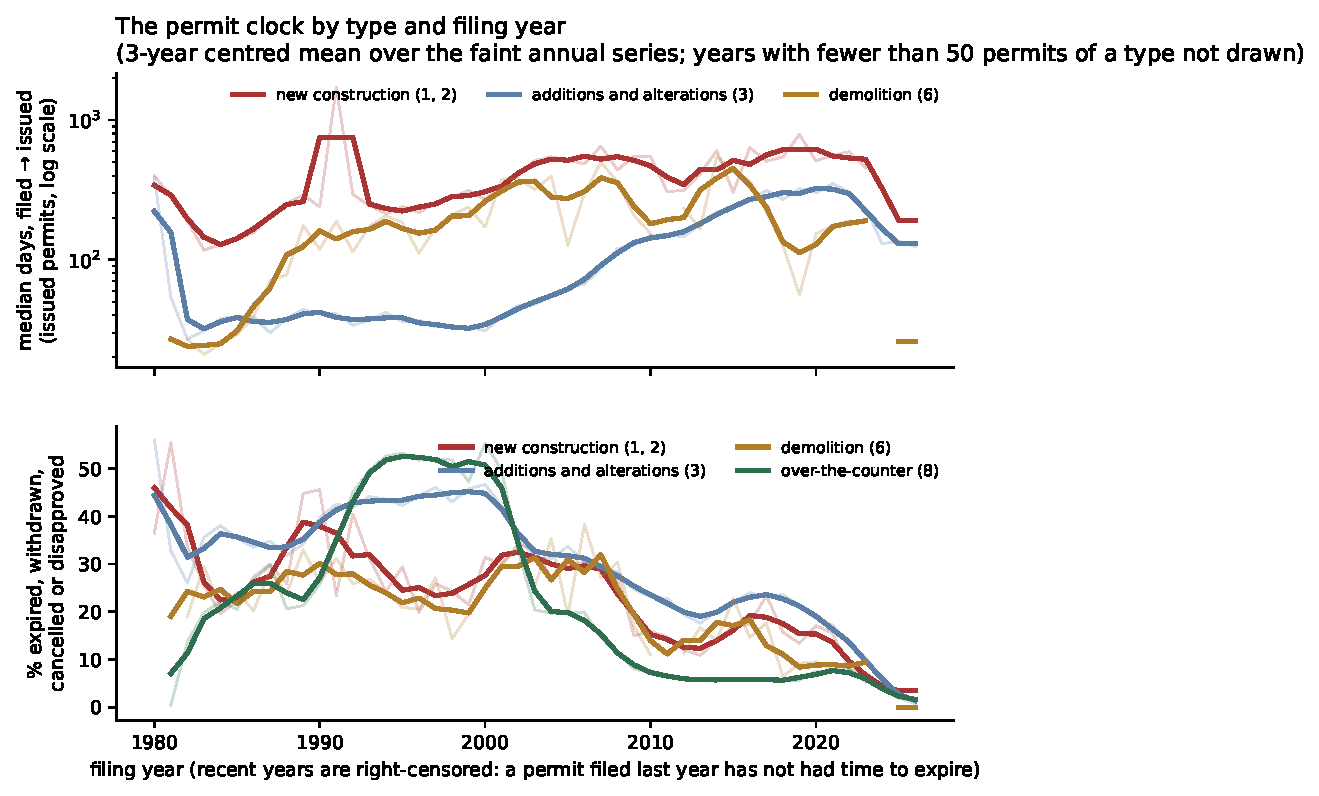
\includegraphics[width=\textwidth]{figures/fig_permit_clock.pdf}
\caption{Top: median days from filing to issuance, by permit type and filing year, among
issued permits; over-the-counter permits are issued the day they are filed and are drawn in
the lower panel only. Bottom: the share of each year's permits that expired, were withdrawn,
cancelled or disapproved. Faint lines are annual values; bold lines a \pcSmoothYears-year
centred mean; years with fewer than \pcMinYearN\ permits of a type are not drawn. The last years are
right-censored in both panels: the permits filed then that are already issued are the fast
ones, and the rest have not had time to expire.}
\label{fig:clock}
\end{figure}

\section{A development-relevant universe}

The question of whether Commission projects differ is not a question about kitchen remodels.
Table~\ref{tab:universe} builds the comparison universe rule by rule and reports what each keeps:
new construction of every construction type, demolitions, site permits, and additions or
alterations that either change the dwelling-unit count or have an estimated cost in the top
\pcCostQ\% of additions and alterations filed the same year. Over-the-counter alterations are
excluded outright. The cost rule is a within-year percentile so that it means the same thing in
1985 and in 2025; a nominal threshold tilts the universe toward recent years, when nominal
costs are higher. The sensitivity rows show the universe under the top \pcCostQAltHi\% and top
\pcCostQAltLo\% and under a nominal \$\pcCostNominal\ million, with the Commission-linked
share of each. The universe holds \pcUniverse\ permits.

\section{Three linkage tiers, kept apart}

Table~\ref{tab:tiers} gives the tiers:

\begin{itemize}
\item \textbf{T1}, a permit number printed in the minutes, parsed and matched exactly as in the
permit-linkage memo: \pcTone\ permits.
\item \textbf{T2}, the Planning Department records' \texttt{building\_permits} field, read
through the case, its parent project record and every record sharing its stem, as in the
data-acquisition memo's bridge: \pcTtwo\ permits. \pcTboth\ are reached both ways.
\item \textbf{T3}, the parcel $+$ type $+$ window rule --- a major permit filed at the item's
parcel between three years before and one year after the hearing. Its precision of
\pcTthreePrecision\ and recall of \pcTthreeRecall\ were measured on discretionary reviews,
where the printed number is ground truth, and are unmeasured anywhere else.
\end{itemize}

\textbf{``Commission-linked'' means T1 or T2.} T3 returns candidate sets whose error rate outside
discretionary review is unknown, so T3-only permits --- \pcTthreeOnly\ of them in the universe
--- are reported as their own group and never pooled with either side of a comparison.

\section{Are Commission projects different?}

Table~\ref{tab:compare} compares the \pcLinked\ Commission-linked permits in the universe with
the development-relevant permits no tier reaches. Each row gives means and medians and the
standardised difference three ways: raw; after reweighting the unlinked group to the linked
group's distribution over cells of permit type $\times$ \pcYearBin-year filing bin $\times$
analysis neighbourhood (\pcSupportCells\% of linked permits have a counterpart cell); and after
reweighting over type $\times$ filing bin $\times$ unit-count bin (\pcSupportUnits\%).
Table~\ref{tab:byunits} repeats the outcome comparison within unit-count bins.

\begin{itemize}
\item \textbf{Era is the first difference, and cells remove it by construction.} Linked permits
were filed on average in \pcLinkedFy\ against \pcUnlinkedFy: both linkage routes reach recent
permits better than old ones. Every raw difference in the table is partly this.
\item \textbf{Scale.} Linked permits cost more: \pcSdLogCostRaw\ standard deviations in log
cost raw, \pcSdLogCostCell\ within cells, \pcSdLogCostUnits\ within unit-count cells.
Proposed units differ by \pcSdUnitsRaw\ raw and \pcSdUnitsCell\ within cells. Some of the gap
is where and when; the rest is that a project large enough to need a hearing is large.
\item \textbf{Time.} Filing to issuance is where the linked group stands apart: \pcSdDaysRaw\
raw, \pcSdDaysCell\ within cells and \pcSdDaysUnits\ within unit-count cells.
Table~\ref{tab:byunits} shows the gap in every unit-count bin. A project that appears in the
minutes takes markedly longer from filing to permit than a similar project in the same
neighbourhood and period that does not --- which is the sign the real-options frame predicts
for the cost of discretion, and which this table describes without identifying.
\item \textbf{Abandonment.} Linked permits expire or are withdrawn less often
(\pcLinkedExit\% against \pcUnlinkedExit\%; \pcSdExitCell\ within cells). A project that has
been through a hearing has sunk more by the time it holds a permit, and a project that would be
abandoned may be abandoned before it ever reaches one.
\item \textbf{Use and place.} Linked permits are more often apartments and less often offices
or one-family dwellings, and more often in residential-house and neighbourhood-commercial
districts at filing; within cells these differences mostly vanish, because the cells hold
place and type fixed.
\end{itemize}

\begin{figure}[htbp]\centering
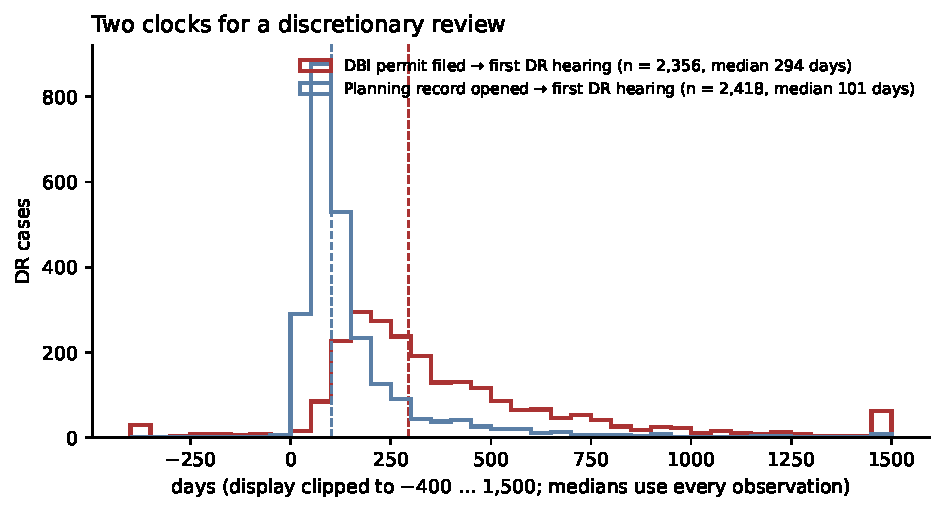
\includegraphics[width=\textwidth]{figures/fig_dr_clock.pdf}
\caption{The two clocks on the discretionary-review track, one observation per DR case. The
display is clipped; the medians use every observation.}
\label{fig:drclock}
\end{figure}

\section{Three targeted comparisons}

Table~\ref{tab:targeted} gives three narrower comparisons, each reweighted over the cells it
names.

\paragraph{The DR track, as a proxy.} The brief asked for noticed permits that drew a DR request
against noticed permits that did not. \textbf{The Planning records do not identify \S311
notification records}: no record type is a notice, and the text mentions notice mostly to say
it was not required. What the records do identify is the DR request, whose description names
its permit from \pcDrpYears; \pcDrpNamed\ of the \pcDrpN\ requests opened in those years do,
and \pcDrNamedInDbi\ of the named permits are major permits in DBI. They are compared with the
other major permits filed \pcDrFiled\ in residential districts, where notice applies. That is a
comparison of permits that drew a DR request against permits that could have, not against
permits known to have been noticed, and it is labelled a proxy wherever it appears.

\paragraph{The CU track.} Permits linked to a conditional use, against development-relevant
permits of the same proposed use in the same zoning district at filing, in the same filing
period, with no Commission link.

\paragraph{Ministerial against Commission, 2018 on.} New construction approved under SB~35 ---
flagged on \pcSbThirtyFive\ project records --- or SB~423, which has no field and is found in
\pcSbFourTwoThree\ records only by its name in the text, reaches \pcMinisterialPermits\ permits
in DBI, against \pcMinCommissionPermits\ Commission-linked new-construction permits of the same
period, reweighted over unit-count bins. The ministerial group is too small for its percentages
to carry weight, and the table says so by giving the counts.

\section{Bunching at the thresholds}

Figure~\ref{fig:bunching} and Table~\ref{tab:bunch} give proposed units from 1 to 40 for every
development-relevant permit and for the Commission-linked ones, before and after
\pcPropC\ (Proposition~C raised the inclusionary requirement that year). The lines mark the
inclusionary threshold at \pcInclusionary\ units, the Transportation Sustainability Fee's
residential tiers --- which begin, as the fee register prints them, at \pcTsfBands\ units ---
and \pcOrdinanceUnits\ units, the brief's figure for the July 2026 ordinance, which this memo
has not checked against the ordinance and which too few 2026 permits exist to test.

Read as counts, the distribution has visible heaping at round numbers in both periods, and the
counts just below and just above each threshold are in Table~\ref{tab:bunch} so the reader can
judge. No bunching estimate is attempted here: the counts near any single threshold are in the
tens, the Commission-linked counts in single digits, and a proposed unit count on a permit is
not the same object as the count at entitlement.

\begin{figure}[htbp]\centering
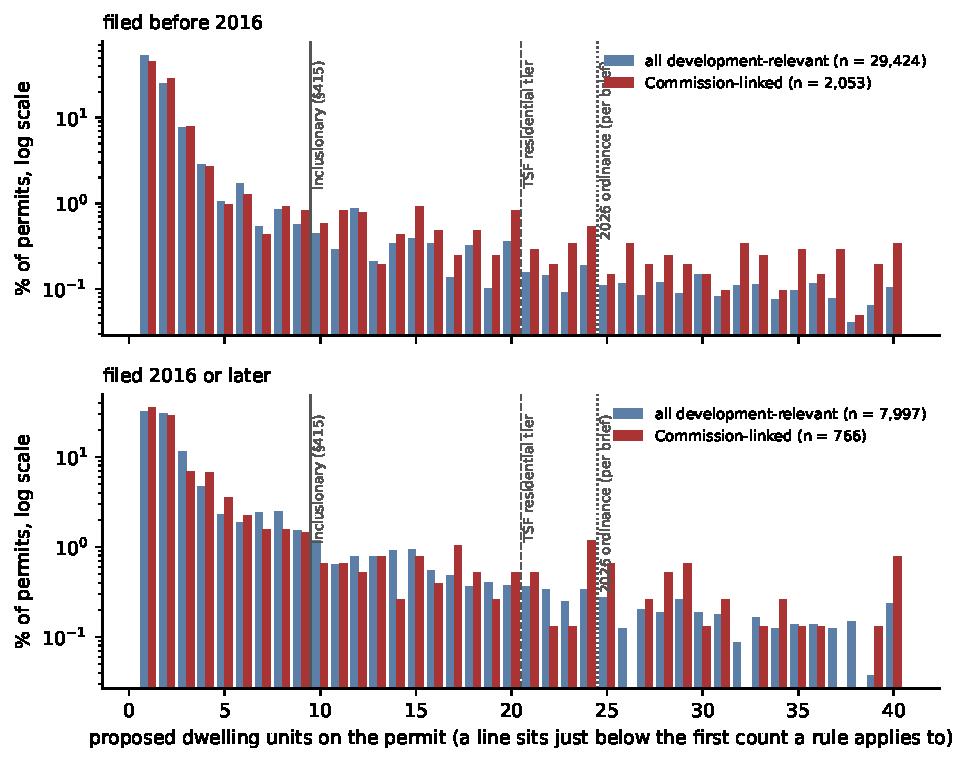
\includegraphics[width=\textwidth]{figures/fig_bunching.pdf}
\caption{Proposed dwelling units on development-relevant permits, 1 to 40, as a share of each
group, on a log scale; before and after \pcPropC. The solid line sits just below the
inclusionary threshold, the dashed lines below the TSF residential tiers, the dotted line
below the brief's 2026 threshold.}
\label{fig:bunching}
\end{figure}

\section{The developer's clock on the DR track}

The data-acquisition memo measured filing to first hearing from the opening of the Planning
record. For a discretionary review that record is the DR request --- filed by a neighbour
against a pending permit --- so the clock starts when the neighbour acts, not when the developer
does. Table~\ref{tab:drclock} and Figure~\ref{fig:drclock} measure the developer's clock
instead: from the DBI filing of the permit the review is about, reached by T1 or T2, to the
first DR hearing. On \pcDrDbiN\ of the \pcDrCases\ DR cases it is a median \pcDrDbiMed\ days
with a 90th percentile of \pcDrDbiPninety; the Planning-record clock on \pcDrRecN\ cases is a
median \pcDrRecMed\ with a 90th percentile of \pcDrRecPninety. On the \pcDrBothN\ cases with
both, the developer's clock is a median \pcDrDiffMed\ days longer. \pcDrDbiNeg\% of the
developer's clocks are negative --- the linked permit was filed after the first hearing ---
and they are kept rather than trimmed.

\section{Caveats}
\label{sec:caveats}

\begin{itemize}
\item \textbf{Duplicate permit numbers.} \pcRowsRepeating\ rows repeat a permit number already
in the table, spread over \pcPermitsRepeating\ permits --- one row per lot a permit touches.
Every count here is on one row per permit, the earliest filed. DBI marks one row per permit
itself (\texttt{primary\_address\_flag}); the two rules pick the same row for \pcRulesAgree\%
of permits, and the choice barely matters for what is compared here: type, cost, units,
dates and status differ between a permit's rows for at most \pcFieldsDiffer\% of the
permits that repeat.
\item \textbf{T3 is unvalidated outside discretionary review}, and is never pooled.
\item \textbf{Coverage rises with era.} Both Commission-linkage routes reach recent permits
better than old ones, which is why every comparison is repeated within filing-period cells.
\item \textbf{Linked does not mean the permit the hearing was about.} T2 in particular reads
every record sharing a case stem, so a large project's linked set can include permits for other
phases or parcels of the same project. The comparison is of permits connected to a Commission case, not of the single permit
each hearing decided.
\item \textbf{The unlinked group is not a control group.} It is the set of development permits
no route reaches, which includes Commission projects whose link is missing. If the missing
links resemble the found ones, the differences are understated rather than overstated; either
way they are descriptions, not effects.
\end{itemize}

\section{Established, and not established}

\textbf{Established.}
\begin{enumerate}
\item The table's \pcCols\ columns, their fill by decade, and \pcNoted\ columns whose rows do not
deliver what the name suggests, including the absence of construction-start dates before the
late 1990s.
\item A development-relevant universe of \pcUniverse\ permits under stated rules, reported
beside three alternative cost rules.
\item Commission-linked development permits take longer from filing to issuance than similar
unlinked permits in the same place, period and type, by \pcSdDaysCell\ standard deviations,
and the gap holds within every unit-count bin; they are larger, and less often abandoned.
\item The developer's clock on the DR track runs a median \pcDrDiffMed\ days longer than the
Planning-record clock.
\end{enumerate}

\textbf{Not established.}
\begin{enumerate}
\item Anything causal. The within-cell differences describe who reaches the Commission; they
do not say what the hearing did.
\item Which of a linked set is the permit the hearing decided.
\item The \S311 comparison as the brief framed it: notices are not in the records.
\item Whether the ministerial group, at \pcMinisterialPermits\ permits, is large enough to say
anything.
\item Any response to the 2026 threshold.
\end{enumerate}

\section{Reproducing this}

\begin{verbatim}
python analyze_permit_content.py fetch            # every column, resumable
python analyze_permit_content.py fetch --refresh  # re-download
python analyze_permit_content.py report           # figures, tables, macros
\end{verbatim}

\texttt{fetch} pages DataSF's Building Permits on the system row identifier into one file per
page under \texttt{\$MFHR\_DATA\_ROOT/external/datasf/dbi\_full\_parts/} and stacks them into
\texttt{dbi\_permits\_full.csv.gz}, with its retrieval time and column list beside it.
\texttt{report} imports the printed-permit parser, the parcel rule and its window from
\texttt{analyze\_permits.py}, and the case normalisers, the planning records and the
\texttt{building\_permits} bridge from \texttt{acquire\_external\_data.py}; it joins the zoning
district in force at filing from the parcel-year panel, reads the fee register for the TSF
tiers, and writes the three figures, \texttt{tables/permits\_content\_tables.tex} and
\texttt{tables/permits\_content\_macros.tex}. The linkage tiers are cached beside the DBI file
and rebuilt whenever it is newer. The only numerals typed into the \texttt{.tex} are section
references, identifiers, the twenty-two columns of the earlier cache, and the legal facts named
as such (Proposition~C, SB~35, SB~423, \S311, the 1985 and 2025 of an example).

\end{document}
